
\section{Conclusiones}

\subsection{PageRank}

A medida que fuimos investigando y probando el algoritmo del PageRank nos fue quedando cada vez más claro como es que funciona y que se necesita para obtener un buen resultado para un sitio en particular.
Lo que nos pareció interesante es explicar el algoritmo con la siguiente interpretación metafórica:

\begin{figure}[h!]

       
\includegraphics[width=0.45\textwidth]{imagenes/pagerank-pipe-goldfish.png}
           \hfill
        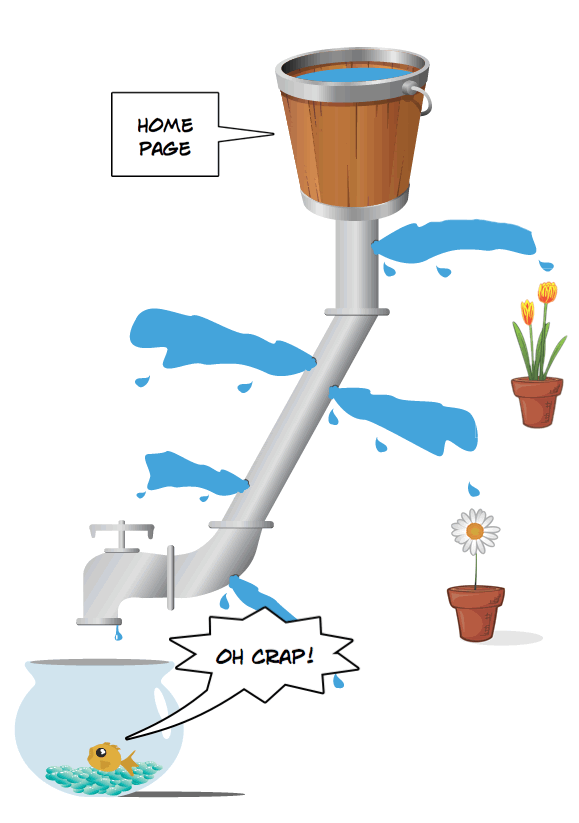
\includegraphics[width=0.45\textwidth]{imagenes/ohcrap-goldfish-flowers.png}

\end{figure}

\FloatBarrier

Tomando como al sitio a analizar en cuestión como la pecera, y a otro sitio que tiene un link a nuestro sitio como el balde se puede observar que cuando el $\textit{recurso}$, en este caso el agua, se reparte equitativamente a todos los destinatarios, por lo tanto, si mi pecera es la única que recibe agua voy a obtener más que si tiene otras bocas la canilla con la cual compartir. Esto es lo mismo que sucede en la web y tiene el cuenta el PageRank, cada sitio le distribuye equitativamente una probabilidad a cada salida, cuya suma total es 1. Por lo tanto, me conviene más que me linkee un sitio con pocas salidas que uno con gran cantidad, pero suponiendo que sus respectivos PageRank son similares, ya que mi PageRank también va a depende del de mis entradas, por lo tanto también hay que tener esto en cuenta, ya que es un factor bastante influyente. Por consiguiente, no solo depende la cantidad de sitios que apuntan a si no también el PageRank de cada uno (la  $\textit{calidad}$)

\newpage


\subsection{HITS}

En el gráfico que nos muestra el tiempo de computo en función del tamaño de los grafos podemos observar que para grafos grandes este algoritmo se vuelve bastante ineficiente. Sin embargo no debemos olvidar que en su paper$[2]$ Kleinberg habla de que este algoritmo debe ser aplicado no sobre toda la red sin sobre un subconjunto de la misma ($\textit{root set}$) obtenido de una busqueda incial. Por lo tanto si acotamos el análisis a los grafos mas acotados podemos ver que el tiempo de computo es aceptable y hasta muy parecido al de page rank. 

\subsection{INDEG}

Este algoritmo es bastante simple y en una red chica y confiable puede llegar a valer. Igualmente tiene mucho peso la confiabilidad, ya que es muy simple de crecer tu puntaje, simplemente comprando un lugar mínimo en la mayor cantidad de páginas posibles. Volviendo al ejemplo anterior, notar que al tener todas las páginas el mismo peso, el nodo dos gana más puntaje simplemente por comprar espacio en las páginas 1, 3, 6 y 7, sin importar qué importancia tengan estas en el resto de la red.

 \begin{figure}[!htb]
\begin{center}
    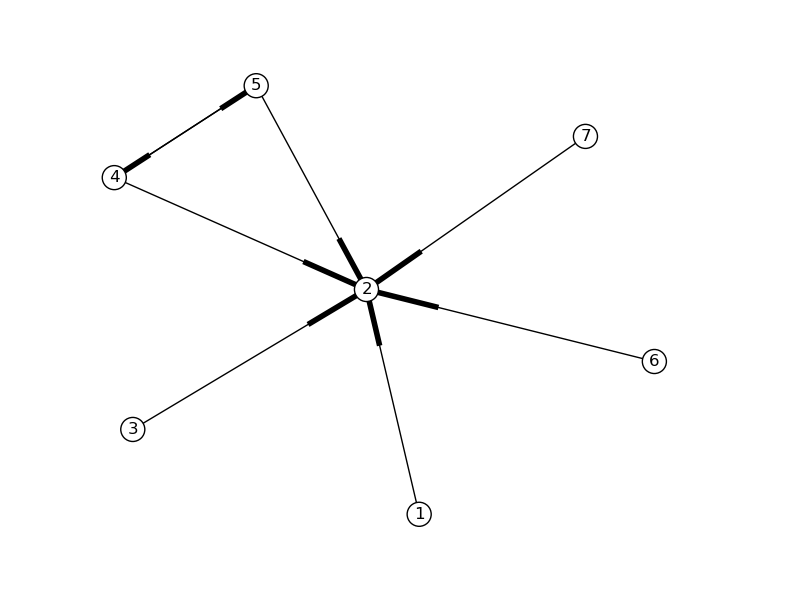
\includegraphics[scale=0.5]{imagenes/test4.png}
    \caption{Red de 7 nodos}
    \end{center}
\end{figure}

\subsection{Mejor estrategia para comprar links}
\subsubsection{PageRank}

Como explicamos anteriormente, el algoritmo de PageRank prioriza la calidad del sitio de entrada antes que la cantidad. Por lo tanto supongamos que tenemos el siguiente escenario:


 \begin{figure}[!htb]
\begin{center}
    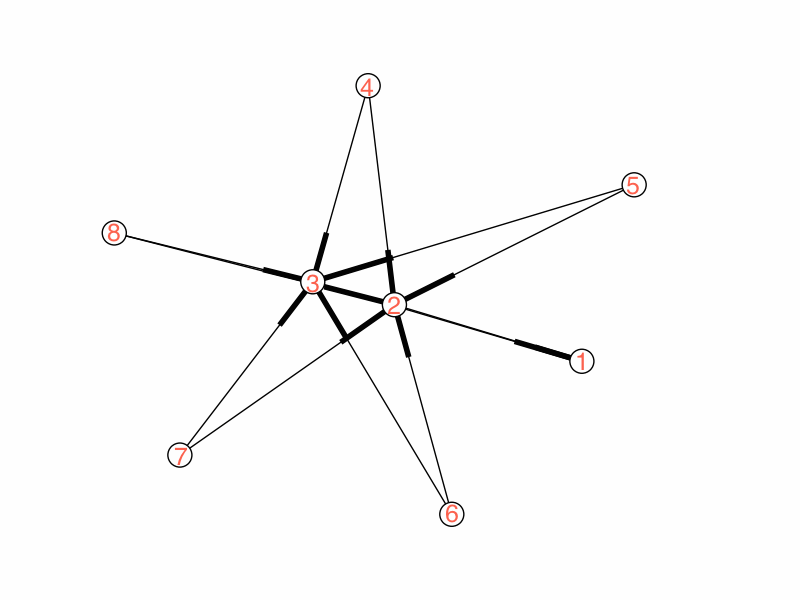
\includegraphics[scale=0.5]{imagenes/test6.png}
    \caption{Red de 8 nodos, c=0.85}
    \end{center}
\end{figure}

Cuyos pesos son:
   $$ 
\begin{bmatrix}
Nodo 1 & 0.32079\\
Nodo 2 & 0.15762\\
Nodo 3 & 0.15762\\
Nodo 4 & 0.05283\\
Nodo 5 & 0.05283\\
Nodo 6 & 0.05283\\
Nodo 7 & 0.05283\\
Nodo 8 & 0.05283\\
\end{bmatrix} 
$$

Ahora, suponiendo que el costo de cada nodo es mas caro a medida que aumenta su peso, vamos a ver que es más conveniente, si comprar el derecho a que el nodo 1 nos apunte o en vez de eso comprar el linkeo de los nodos 2 y 3. Entonces vamos a testear como se comporta el algoritmo mediante estas dos alternativas lineando al sitio de los Wachiturros.


   $$ 
\begin{bmatrix}
 & Nodo 1 & Nodo 2 y 3 \\
Wachiturros & 0.24557  & 0.05018   \\
Nodo 1 & 0.24201& 0.30469\\
Nodo 2 & 0.11891& 0.14971\\
Nodo 3 & 0.11891& 0.14971\\
Nodo 4 & 0.03986  & 0.05018\\
Nodo 5 & 0.03986  & 0.05018\\
Nodo 6 & 0.03986  & 0.05018\\
Nodo 7 & 0.03986 & 0.05018\\
Nodo 8 & 0.03986 & 0.05018\\
\end{bmatrix} 
$$

Por lo tanto se puede ver que conviene que el Nodo 1 nos apunte antes que el 2 y 3. Conviene porque nos asigna un mayor peso y porque nos deja a su vez mejor posicionado en la tabla final. Además de significar una optimización en el costo total.

\subsubsection{HITS}
Si el algoritmo aplicado en la red fuese HITS lo recomendable al cliente sería que neogice con los principales HUBS para que apunten a su sitio. Logrando así rankear mejor en la sección de Autoridades sobre el tema. No le recomendaríamos que negocie con las páginas autoridades ya que dificilmente estas accediesen ya que de esta manera se estarían restando puntos en el ranking de autoridades.
